\documentclass[12pt]{article}
\usepackage[utf8]{inputenc}

\usepackage[margin=1in]{geometry}
\usepackage{color,soul}
\usepackage{xcolor}
\usepackage{array}
\usepackage{mhchem}
\usepackage{mathtools}

\DeclarePairedDelimiter\ceil{\lceil}{\rceil}
\DeclarePairedDelimiter\floor{\lfloor}{\rfloor}

\bibliographystyle{plos2015}


\begin{document}


\vspace*{0.2in}

% Title must be 250 characters or less.
\begin{flushleft}
{\Large
\textbf\newline{Adaptive dating and fast proposals: revisiting the phylogenetic relaxed clock model} % Please use "sentence case" for title and headings (capitalize only the first word in a title (or heading), the first word in a subtitle (or subheading), and any proper nouns).
}
\newline
% Insert author names, affiliations and corresponding author email (do not include titles, positions, or degrees).
\\
Jordan Douglas\textsuperscript{1,2*},
Rong Zhang\textsuperscript{1,2},
Remco Bouckaert\textsuperscript{1,2,3}
\\
\bigskip
\textbf{1} Centre for Computational Evolution,  University of Auckland, Auckland, New Zealand\\
\textbf{2} School of Computer Science, University of Auckland, Auckland, New Zealand\\
\textbf{3} Max Planck Institute for the Science of Human History, Jena, Germany\\
\bigskip


% Use the asterisk to denote corresponding authorship and provide email address in note below.
* jordan.douglas@auckland.ac.nz


\end{flushleft}


\section*{S3 Appendix: Supplementary results}





\begin{figure}[!htb]
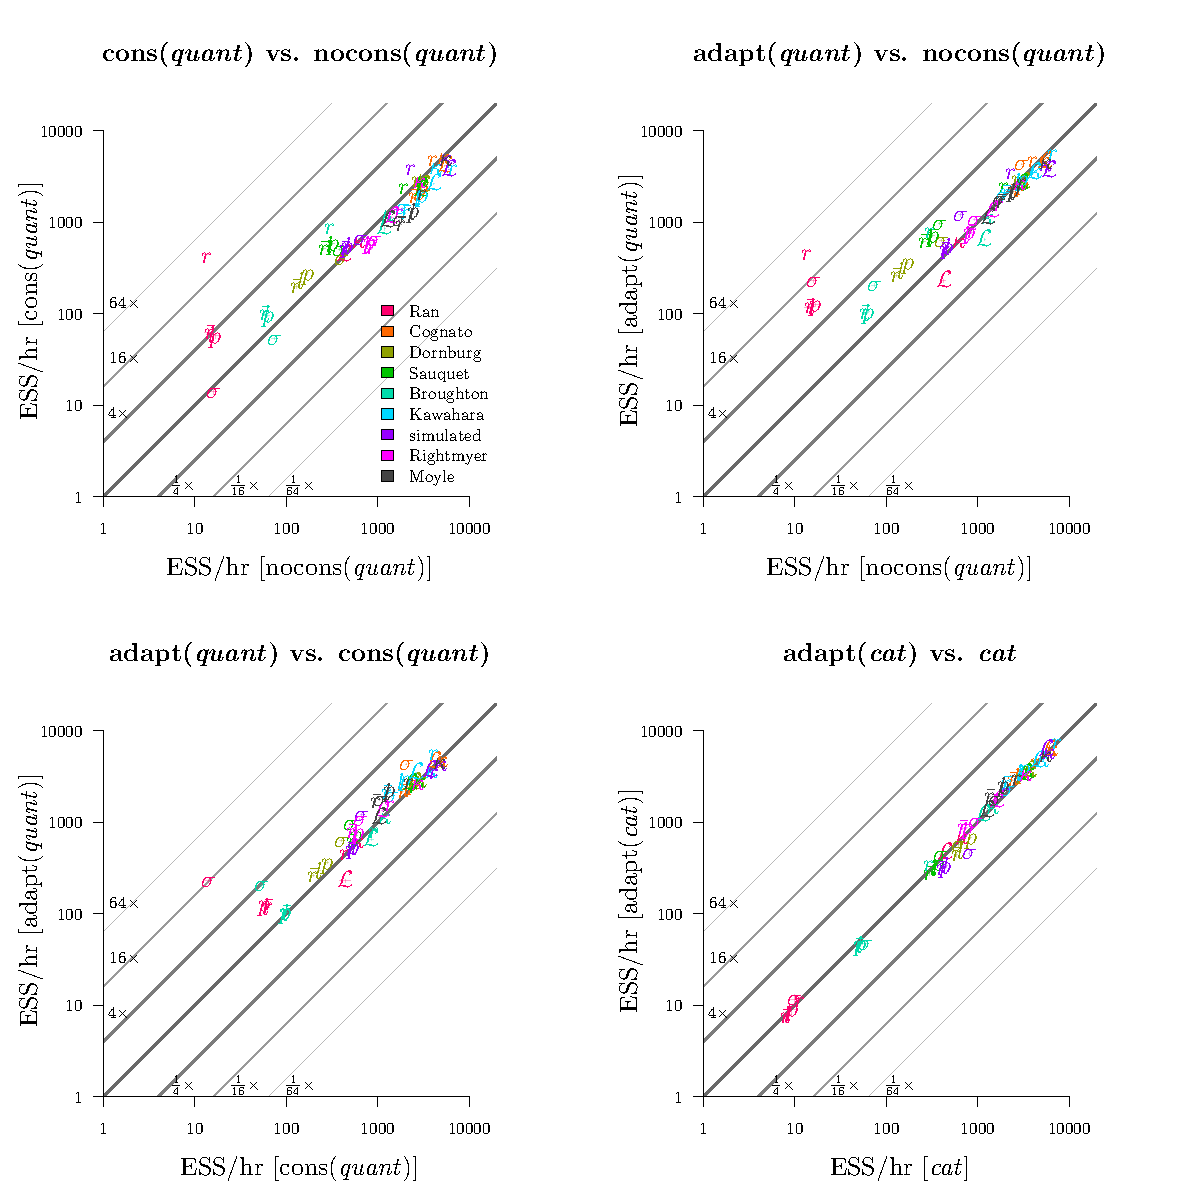
\includegraphics[width=\textwidth]{benchmarking/benchmarkingVM/ESS_round1_catquant.pdf}
\caption{\textbf{Round 1: Performance evaluation of \texttt{AdaptiveOperatorSampler} under the \emph{quant} and \emph{cat} parameterisations.}
These results show that \emph{cat} does not benefit from adaptive weight sampling. Whereas, adapt and cons both greatly improve the \emph{quant} parameterisation for most datasets, as expected. }
\end{figure}







%\bibliography{references}




\end{document}